\documentclass[tikz]{standalone}

\begin{document}

\bfseries
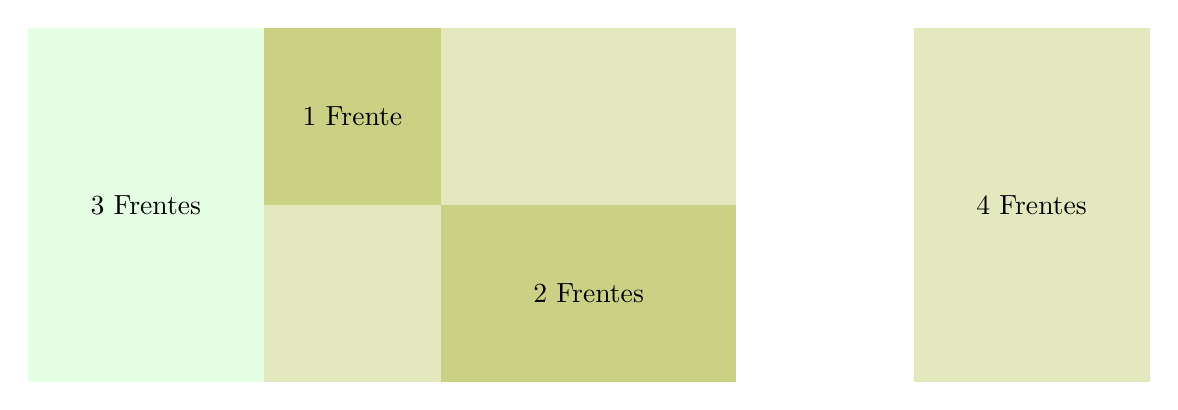
\begin{tikzpicture}[scale=1.5]
	\fill [green!10] 
	(0,0) rectangle node [text=black] {3 Frentes} (2,3);
	\fill [olive!80!green!20!white] 
	(2,0) rectangle ++(4,3);
	\fill [olive!80!green!20!white] 
	(7.5,0) rectangle node [text=black] {4 Frentes} ++(2,3);
	\fill [olive!80!green!40!white] 
	(2,1.5) rectangle node [text=black] {1 Frente} ++(1.5,1.5);
	\fill [olive!80!green!40!white] 
	(3.5,0) rectangle node [text=black] {2 Frentes} ++(2.5,1.5);
\end{tikzpicture}

\end{document}
